\documentclass[12pt]{article}
\usepackage[utf8]{inputenc}
\usepackage[spanish]{babel}

\usepackage{graphicx}



\title{WordNet en Prolog}
\author{Alejandro Camacho Pérez\\Grupo C-312}

\date{}

\begin{document}

\maketitle
\tableofcontents

\section{Resumen}

En este trabajo se ha implementado una interfaz en Python para acceder a la base de datos de WordNet en Prolog, de forma que se puedan realizar consultas de forma sencilla y obtener los resultados de forma legible. Para ello se ha utilizado la librería \texttt{pyswip} que permite la comunicación entre Python y Prolog, así cómo la librería \texttt{tkinter} para la interfaz gráfica. \\

La interfaz permite realizar 11 tipos de consultas diferentes, que se describen en la sección \ref{sec:consultas}. Para cada una de ellas se ha implementado una función en Python que se encarga de realizar la consulta en Prolog y devolver los resultados.

\newpage

\section{Descripción}

\subsection{Interfaz gráfica}

% Load ui.png

\begin{figure}[h]
    \centering
    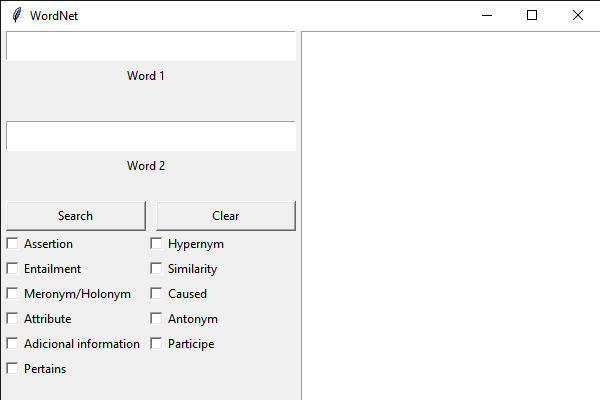
\includegraphics[width=0.8\textwidth]{ui.png}
    \caption{Interfaz gráfica}
    \label{fig:ui}
\end{figure}

La interfaz gráfica se ha implementado utilizando la librería \texttt{tkinter} de Python. Se ha creado una clase GUI que contiene todos los elementos de la interfaz, y que se inicializa en el fichero \texttt{main.py}. \\
La interfaz se divide en tres partes:

\newpage

\subsubsection{Entrada de datos:}

% Load entry.png

\begin{figure}[h]
    \centering
    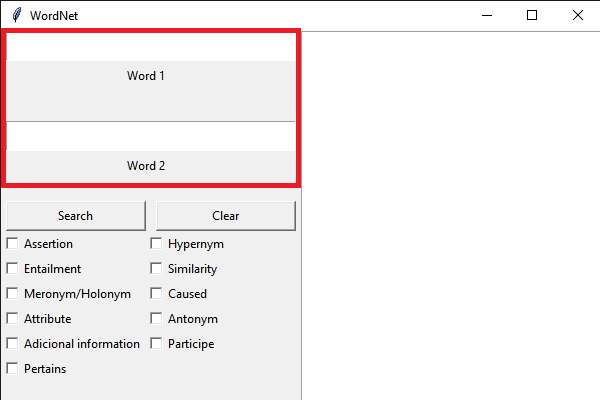
\includegraphics[width=0.8\textwidth]{entry.png}
    \caption{Entrada de datos}
    \label{fig:entry}
\end{figure}

En esta parte se introducen los datos necesarios para realizar la consulta. El tipo de consulta determina los datos que se deben introducir. Por ejemplo, para la consulta \texttt{hiperónimos} se debe introducir un sustantivo, mientras que para la consulta \texttt{antónimos} se debe introducir un adjetivo. El programa no permite realizar consultas con datos incorrectos, es decir, si se introduce un adjetivo en una consulta que requiere un sustantivo, se mostrará un mensaje de error.

\newpage

\subsubsection{Botón de consulta:}

% Load buttons.png

\begin{figure}[h]
    \centering
    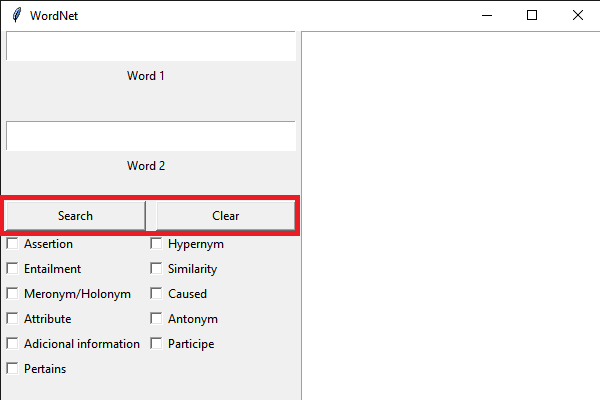
\includegraphics[width=0.8\textwidth]{buttons.png}
    \caption{Botón de consulta}
    \label{fig:buttons}
\end{figure}


El botón \texttt{Search} se utiliza para realizar la consulta con los datos introducidos y el operador seleccionado.\\

El botón \texttt{Clear} se utiliza para limpiar los datos introducidos y los resultados de la consulta.

\newpage

\subsubsection{Resultados:}

% Load text.png

\begin{figure}[h]
    \centering
    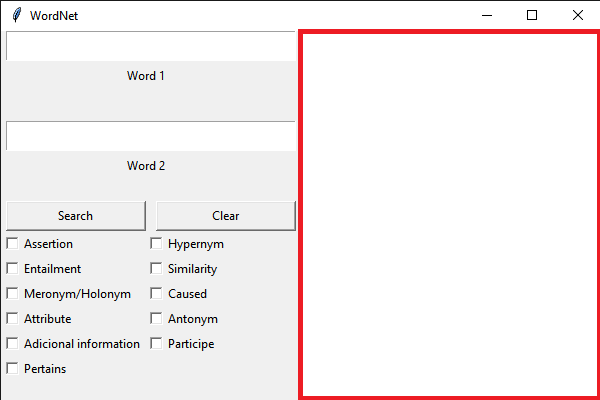
\includegraphics[width=0.8\textwidth]{text.png}
    \caption{Resultados}
    \label{fig:text}
\end{figure}

En esta región se muestran los resultados de la consulta, así como los mensajes de error en caso de que se produzcan.

\newpage

\subsubsection{Operadores}

% Load operators.png

\begin{figure}[h]
    \centering
    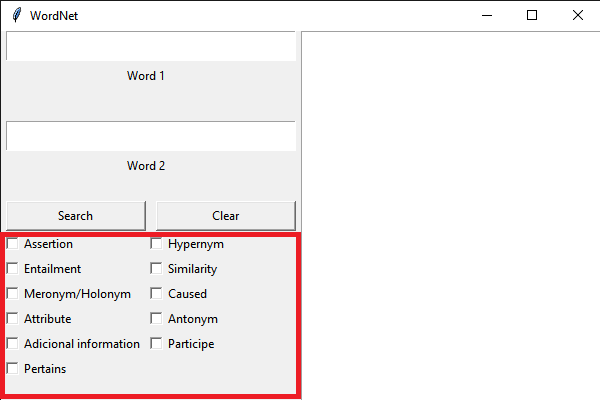
\includegraphics[width=0.8\textwidth]{operators.png}
    \caption{Operadores}
    \label{fig:operators}
\end{figure}

Para poder realizar una consulta, es necesario seleccionar el operador a utilizar, que determina el tipo de consulta que se va a realizar.



\subsection{Consultas}
\label{sec:consultas}

Se han implementado 11 tipos de consultas diferentes, que se describen a continuación. Para cada una de ellas se ha implementado una función en Python que se encarga de realizar la consulta en Prolog y devolver los resultados.

\subsubsection{Assertions}

Se utiliza para encontrar todos los significados posibles de la palabra especificada en la primera entrada.

\subsubsection{Entailment}

Se utiliza para encontrar todos los verbos que se vinculan con el verbo especificado en la primera entrada. Si sólo se especifica la segunda entrada, se utiliza para encontrar todos los verbos de los cuales se deriva de su acción el verbo especificado. En caso de que sean utilizadas ambas entradas, se comprueba si los verbos dados están vinculados.

\subsubsection{Meronym/Holonym}

Se utiliza para encontrar los merónimos o holónimos de la palabra especificada en la primera o la segunda entrada respectivamente. En caso de que sean utilizadas ambas entradas, se comprueba si la palabra especificada en la primera entrada es un merónimo de la palabra especificada en la segunda entrada.

\subsubsection{Attribute}

Se utiliza para encontrar los adjetivos que hacen de atributo al sustantivo especificado en la primera entrada. En caso de que se especifique la segunda entrada, se buscan los sustantivos de los cuales ese adjetivo hace de atributo. Si ambas entradas son especificadas, se comprueba si el adjetivo especificado en la primera entrada hace de atributo al sustantivo especificado en la segunda entrada.

\subsubsection{Aditional information}

Se utiliza para encontrar las palabras que aportan información adicional al verbo o adjetivo especificado en la primera entrada.

\subsubsection{Pertains}

Si en la primera entrada se especifica un adjetivo, el resultado será un sustantivo o adjetivo que se relaciona con el adjetivo especificado. Si en la primera entrada se especifica un adverbio, el resultado será un adjetivo del cual se deriva el adverbio especificado.

\subsubsection{Hypernym}

Se utiliza para encontrar los hiperónimo del sustantivo especificado en la primera entrada. En caso de que se especifique la segunda entrada, se buscan los sustantivos de los cuales el sustantivo especificado en la primera entrada es hiperónimo. Si ambas entradas son especificadas, se comprueba si el sustantivo especificado en la primera entrada es hiperónimo del sustantivo especificado en la segunda entrada.

\subsubsection{Similarity}

Se utiliza para encontrar los adjetivos con significado similar al adjetivo especificado en una de las entradas. Si se especifican ambas entradas, se comprueba si los adjetivos especificados son similares.

\subsubsection{Caused}

Se utiliza para encontrar los verbos que causados por el verbo especificado en la primera entrada. Si se especifica la segunda entrada, se buscan los verbos que causan el verbo especificado en la primera entrada. Si se especifican ambas entradas, se comprueba si el verbo especificado en la primera entrada causa el verbo especificado en la segunda entrada.

\subsubsection{Antonym}

Se utiliza para encontrar los antónimos del adjetivo especificado en la primera entrada. Si se especifica la segunda entrada, se buscan los adjetivos que son antónimos del adjetivo especificado en la primera entrada. Si se especifican ambas entradas, se comprueba si el adjetivo especificado en la primera entrada es antónimo del adjetivo especificado en la segunda entrada.

\subsubsection{Participle}

Se utiliza para encontrar los participios del verbo especificado en la primera entrada. Si se especifica la segunda entrada, se buscan los verbos de los cuales el verbo especificado en la primera entrada es participio. Si se especifican ambas entradas, se comprueba si el verbo especificado en la primera entrada es participio del verbo especificado en la segunda entrada.

\subsection{Implementación}

El proyecto se divide en 3 archivos principales: \texttt{main.py}, \texttt{gui.py} y \texttt{prolog\_api.py}. En el archivo \texttt{main.py} se inicializa la interfaz gráfica y se definen las funciones que se ejecutan al pulsar el botón de consulta. En el archivo \texttt{gui.py} se define la clase GUI que contiene todos los elementos de la interfaz gráfica. En el archivo \texttt{prolog.py} se define la clase Consulter que contiene las funciones que se encargan de realizar las consultas en Prolog.

\subsubsection{gui.py}

Este código en Python es una implementación de una interfaz gráfica de usuario (GUI) utilizando la biblioteca \texttt{tkinter} para consultas en un programa basado en Prolog (se hace referencia a \texttt{prolog\_api}). La interfaz consta de botones de selección (\texttt{CheckButton}) que representan diferentes opciones y dos campos de entrada de texto para ingresar palabras. Además, se incluyen botones de búsqueda (\texttt{Search}) y limpieza (\texttt{Clear}), junto con un área de texto para mostrar los resultados.

\begin{enumerate}

    \item Se importan las bibliotecas necesarias, como \texttt{Enum} de \texttt{enum}, \texttt{tkinter} y algunos elementos personalizados (\texttt{Consulter} y \texttt{Operator}).

    \item Se define la clase \texttt{GUI} que representa la interfaz de usuario. El constructor \texttt{\_\_init\_\_} inicializa varios atributos y crea la ventana principal de la interfaz.

    \item El método \texttt{run} inicia el bucle principal de la interfaz gráfica (\texttt{mainloop}).

    \item El método \texttt{place} organiza los elementos gráficos en la ventana según cuadrantes y tamaños relativos.

    \item Se definen métodos para el manejo de eventos, como el redimensionamiento de la ventana (\texttt{resize\_result\_text}), la creación de botones de verificación (\texttt{create\_check\_buttons}), y la manipulación del estado de los botones de verificación (\texttt{check\_box\_behavior}).

    \item El método \texttt{select\_text} actualiza la información asociada a las entradas de texto según el estado de los botones de verificación.

    \item El método \texttt{show\_result} actualiza el área de texto con el resultado de una consulta.

    \item Los métodos \texttt{search\_behavior} y \texttt{clear\_behavior} están asociados a los botones de búsqueda y limpieza, respectivamente. El primero realiza una consulta al sistema basado en Prolog y actualiza la interfaz con el resultado. El segundo restablece el estado de la interfaz a valores iniciales.

\end{enumerate}

\subsubsection{prolog\_api.py}

En el archivo \texttt{prolog\_api.py} se definen las clases \texttt{Consulter}, \texttt{Operator} y \texttt{WordInfo}. \\

La clase \texttt{Consulter} se encarga de realizar las consultas en Prolog. Para ello utiliza la librería \texttt{pyswip} que permite la comunicación entre Python y Prolog. En el constructor de la clase, se inicializa el objeto \texttt{Prolog} que se encarga de realizar las consultas, y se cargan en memoria los archivos de la base de datos de WordNet con el método \texttt{load\_consults}. Para realizar una consulta a la base de datos, se cuenta con el método \texttt{receive\_query} que recibe como parámetro el operador a utilizar y las palabras de la consulta. Esta query es almacenada en la clase para su posterior uso por el  método \texttt{process\_query} que se encarga de obtener los resultados de la consulta. \\

Al realizar el llamado para procesar la query, el método primero busca la información necesaria en la base de datos de ambas palabras introducidas, para luego seleccionar segun el operador, que metodo se utilizará para procesar la query. Cada metodo devuelve un string con los resultados de la consulta, que es luego almacenado en la variable \texttt{result\_string} de la clase, de forma tal que siempre se puede acceder al último resultado procesado. Para corregir errores de paralelismo de la librería \texttt{pyswip}, se utiliza el método \texttt{make\_consult}, quien recibe el string a consultar a los archivos prolog, y espera a que el resultado sea procesado para devolverlo en una lista. \\

Los métodos específicos para procesar cada tipo de consulta, siguen el siguiente patrón: \\

\begin{enumerate}

    \item Comprueban si las palabras introducidas son válidas, es decir, si se encuentran en la base de datos. En caso de que no lo sean, se devuelve un mensaje de error.
    \item Se crea la query a consultar en Prolog, utilizando los datos obtenidos de la base de datos.
    \item Se realiza la consulta en Prolog utilizando el método \texttt{make\_consult}.
    \item Se procesa la lista devuelta para dar un resultado legible y claro.
    \item Se devuelve el resultado.

\end{enumerate}

Los métodos utilizados son:

\begin{itemize}
    \item \texttt{assertion()}
    \item \texttt{similarity\_1\_to\_2()}
    \item \texttt{similarity\_1\_to\_all(word\_selector)}
    \item \texttt{antonym\_1\_to\_2()}
    \item \texttt{antonym\_1\_to\_all(word\_selector)}
    \item \texttt{is\_hypernym()}
    \item \texttt{hypernym\_of()}
    \item \texttt{inverse\_hypernym()}
    \item \texttt{is\_entailment()}
    \item \texttt{entailment\_of()}
    \item \texttt{inverse\_entailment()}
    \item \texttt{is\_meronym\_holonym()}
    \item \texttt{mer\_hol(function,operator)}
    \item \texttt{caused()}
    \item \texttt{is\_attribute()}
    \item \texttt{attribute\_of(word\_selector)}
    \item \texttt{sa()}
    \item \texttt{is\_participle()}
    \item \texttt{participle\_of(word\_selector)}
    \item \texttt{pertains()}
\end{itemize}

Cada uno de ellos está bien documentado en el código.\\

El enum \texttt{Operator} se utiliza para almacenar los operadores disponibles.

La clase \texttt{WordInfo} es una representación de la información asociada a una palabra en WordNet. Esta clase tiene diversos atributos que almacenan detalles como los identificadores de synsets (\texttt{synset\_id\_list}), tipos de palabra (\texttt{word\_type\_list}), números asociados por cada synset (\texttt{word\_number\_list}), grado de sensibilidad de la palabra (\texttt{word\_sense\_list}), significado de la palabra en un synset (\texttt{gloss\_list}), cantidad de veces que aparece la palabra (\texttt{tag\_count\_list}), y un indicador booleano (\texttt{exist}) que señala si la palabra existe o no en la base de datos.

El constructor \texttt{\_\_init\_(self, word: str)} inicializa la instancia de la clase, tomando la palabra como parámetro y asignándola al atributo \texttt{word}. Los demás atributos se inicializan como listas vacías y el indicador de existencia se establece en \texttt{False}.

El método \texttt{\_\_str\_(self)} proporciona una representación de cadena de la palabra, devolviendo simplemente el valor del atributo \texttt{word}.

\subsubsection{main.py}

El archivo \texttt{main.py} es donde se crea la instancia de la clase \texttt{GUI} y se ejecuta el método \texttt{run} para iniciar la interfaz gráfica.

\section{Bibliografía}

\begin{itemize}
    \item Sarah Witzig 'Accessing WordNet from Prolog' (2003)
    \item Documentación de WordNet
\end{itemize}

\end{document}
